\chapter{Solution} \label{chap:solution} \minitoc

\section*{}

This chapter describes how the problem presented in Chapter \ref{chap:problem_statement} was solved by stating the solution implemented and the reasons for the choices taken.  \textbf{\textcolor{red}{End with the sections' descriptions}}

\section{Overview}\label{sec:solution_overview}

The goal of this dissertation is to modify Node-RED in order to decentralize its architecture, taking advantage of the capabilities of external devices, no matter how limited they are.

The solution implemented was to use the Node-RED instance to orchestrate the decentralization and send tasks to other devices in the network. The devices make themselves known by announcing their address and capabilities to a registry node running in Node-RED. Consequently, Node-RED assigns nodes to devices and communicates each node's assignment via WiFi. Due to the devices' limitations, they cannot run an instance of Node-RED, so Node-RED needs to convert nodes in Javascript to other language that can be interpreted by these devices. The implemented solution requires a Micropython port and a HTTP server that receives and executes a micropython script created by the Node-RED. This script contains the tasks assigned to a device, translated into micropython. 

After the first deployment of the system, the Node-RED instance manages the state of each device, allowing the system to re-orchestrate if any of the devices becomes unavailable.

\begin{figure}[h]
\centering
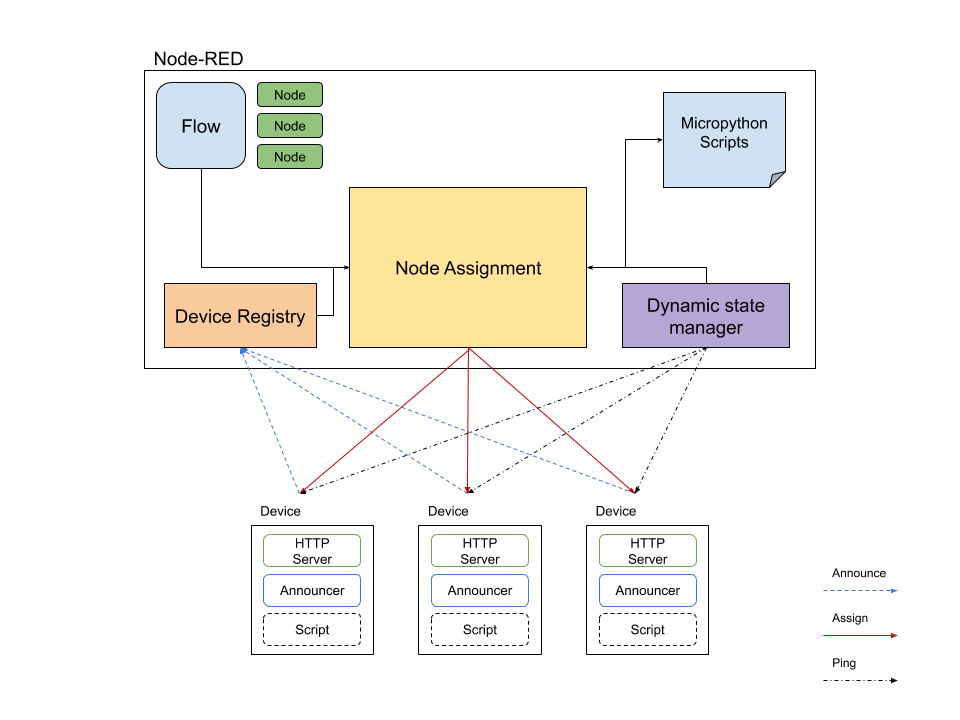
\includegraphics[width=\textwidth]{overview.png}
\caption[Solution's overview]{An overview of the solution}\label{fig:solution_overview}
\end{figure}

\textcolor{blue}{Explain and improve graphic}


\section{Implementation details}\label{sec:implementation_details}

\subsection{Device registry}\label{sec:registry}

When a device becomes available it sends information about itself to a MQTT topic. This information contains the device's IP address, their capabilities and their status - if the device has failed before. In its turn, Node-RED contains a Node called \textit{Registry} that listens to the announcements MQTT topics and saves the devices information. If this node is connected to a orchestrator node, each new device is communicated so that the orchestration can be updated.

When a device has an Out of Memory error, it triggers a fail-safe, where it reboots the HTTP server, stop running any script and restarts all communications. After this action, the device announces itself again but with a flag that indicates that it has failed. This way, Node-RED knows that a device is active but not running any code, and that it possible failed due to too much work. In that case, Node-RED will assign less nodes to the device, reducing the chances of causing another Out of Memory error.

\textcolor{blue}{What is there more to add? Maybe this section is not here, add to other place}

\subsection{Devices setup for decentralization support}\label{sec:devices_decentralization}

The first problem approached in this thesis was finding a way to take advantage of devices with few computational resources, integrating them in a IoT system. The goal was to make these devices execute scripts of code and communicate with other devices, despite their capability limitations. In order to limit the number of type of different devices capable for this aim, only ESP8266 and ESP32 chips were used, since they have connectivity capabilities such as an WiFi chip. In terms of testing, the environment in the devices was replicated in Docker container running the Unix port of micropython.

\subsubsection{Solution overview}

As it was mentioned before in Section \ref{sec:solution_overview}, the devices in the system run a micropython port that allows to run scripts written in micropython. This solution is lightweight and extensible enough that allows to perform several types of tasks. Since these devices need to receive different types of tasks throughout their execution, an HTTP server was implemented, responsible for receiving scripts of code, saving and executes them. Besides this functionality, it was also implemented an endpoint that returns the state of the device, as well as the announcing mechanism, explained in Section \ref{sec:registry}.

Several micropython libraries were used, more specifically uasyncio and micropython-mqtt. The uasyncio library allowed the implementation of asynchronous operations, critical for executing the given code as well as maintaining the HTTP server running and non-blocking.

% It uses micropython and external libraries such as uasyncio and micropython-mqtt.

\textcolor{blue}{Talk about why micropython was chosen, the announcements logic, the server script, the libraries used (mqtt\_as and uasyncio) and the enpoints created for code execution, ping and metrics.}

\subsubsection{Limitations}

\begin{itemize}
    \item Only supports mqtt qos 0 and 1, due to limitation of MQTT library used (the only one that has recent support and more complete)
    \item If a given script is too big, there will be memory problems with ESP8266 -> failsafe not possible
\end{itemize}

\subsection{Node-RED decentralization of computation}\label{sec:node_red_decentralization}

\subsubsection{MQTT node communication support}\label{sec:mqtt_support}

Node-RED nodes communicate using events, where a node only communicates with nodes it is wired to. The communication is one way, with the node only sending data to the nodes it is connected to by output. These output wires are used to access the nodes the message must be sent to, and their \texttt{receive()} method is called. This method triggers the event \texttt{emit} which will the caught by a specific method of each node, implementing its own logic.

\textcolor{blue}{Insert code block with example? Or an image explaining?}

This implementation is local and Javascript specific, making it impossible to be used in a decentralized architecture where nodes will be executed outside the Node-RED instance. It was necessary to implement a way of communicating between nodes external to Node-RED that could be supported by low capacity devices. The solution found was MQTT, which fits as a good solution by its low cost and high popularity.

Node entities were changed to support MQTT instead of events, subscribing to topics created at run-time that match the wires between the nodes. Support for sub-flows was also implemented.

\textcolor{blue}{Insert here image that shows a flow with wires and the respective flow with examples of topics}

\subsubsection{Code generation}\label{sec:code_generation}

\textcolor{blue}{Talk about each node code generation, the support for multiple node scripts in one script. Talk about limitation that different nodes on one script, even consecutive nodes, require to communicate with each other by MQTT topics}

As explained above, due to the limitations of the devices used, it was necessary to translate Node-RED nodes, written in Javascript, to micropython code. Along with that, it was also necessary to support multiple nodes in one script, making it necessary to create a generalized script that could fit any type of node.

The implemented solution consists of each node having specific methods related to their functionality and one point of input and output. Since the communication is made by MQTT, as specified in Section \ref{sec:mqtt_support}, the only input a Node can have is in its topics. The same for the output logic. A exception to this is in nodes that are sources, meaning that they generate input and don't receive it. 

The creation the script is made after the assignment of nodes to devices, and each device has its respective script created. The process consists of creating the script with the code of all the assigned nodes and a general code that ties up the script. This general code is responsible for subscribing to all the input topics of all the nodes, stopping the script's processes and forwarding the MQTT messages to the respective node's code.

\textcolor{blue}{Insert Node-RED flow example and the respective micropython script}

\subsubsection{Custom nodes}\label{sec:custom_nodes}

\textcolor{blue}{temperature-Humidity, if, and, mqtt-in, mqtt-out, orchestrator, registry, failure, nothing}

\subsubsection{Computation Decentralization}\label{sec:node_red_computation_decentralization}

\textcolor{blue}{Talk about the metrics used to assign nodes to devices (predicates and priorities, similar to kubernetes),  the greedy algorithm used to assign nodes to devices. Explain the reassignment if memory errors occurred when sending scripts to the devices or if a device is not responding. Explain when the assignment is made ((a) boot-up after 3 seconds - to give time for the registry to receive all the announcements from the devices, (b) deployment of entire flow, (c) announcement of a new device, (d) failure/recovery of a device with the dynamic state management mechanism}

% node
% bestIndex = 0

% for device in devices:
%     if not all node predicates in device tags: return
%     intersectionIndex = (nº of node priorities in device tags)/(nº node priorities)
    
%     matchIndex = 
%         intersectionIndex * 0.5 + 
%         (1/( nodes assigned to the device) + 1) * 0.4 +
%         (nº of node priorities in device tags/ device tags) * 0.1
    
%     if matchIndex > bestIndex:
%         bestIndex = matchIndex
%         device is the best choice for node

\subsubsection{Dynamic state management}\label{sec:dynamic_state_management}

\textcolor{blue}{Talk about the ping pattern, how the system handles when a device fails or recovers}

\subsubsection{Limitations}\label{sec:limitations}

\begin{itemize}
    \item Number of nodes that support micropython code generation is small
    \item Duplicate messages when redeploying the totality of the flow (maybe fixable later)
    \item Re-orchestration only supported when deploying the entire instance (all flows)
    \item Nodes do not stop working when the Node-RED instance is stopped
    \item \textcolor{blue}{add more}
\end{itemize}
